\documentclass[5p,sort&compress]{elsarticle}	

% THIS IS THE SETUP FROM NIRIS TEMPLATE

\newcommand{\RomanNumeralCaps}[1]
{\MakeUppercase{\romannumeral #1}}
\makeatletter
\def\ps@pprintTitle{%
  \let\@oddhead\@empty
  \let\@evenhead\@empty
  \def\@oddfoot{\footnotesize\itshape
    \hfill\today}%
  \let\@evenfoot\@oddfoot}
\makeatother
\usepackage{dcolumn}
\usepackage[utf8]{inputenc}
\usepackage[T1]{fontenc}

\usepackage{textcomp}
\usepackage{lmodern}
\renewenvironment{abstract}{\global\setbox\absbox=\vbox\bgroup
  \hsize=\textwidth\def\baselinestretch{1}%
  \noindent\unskip\textbf{Abstract}
  \par\medskip\noindent\unskip\ignorespaces}
{\egroup}
\usepackage{amsmath}
\usepackage{amssymb}
\usepackage{caption} %% figurer fugler
\usepackage{bm}
\usepackage{siunitx}
\sisetup{
  exponent-product = \cdot,
  output-decimal-marker  =  {.}, % komma-stil
  separate-uncertainty = false, %true hvis du ikke vil ha usikkerhet i parentes
  per-mode = symbol,
  group-digits = false,
}
\usepackage{graphicx}
\renewcommand{\topfraction}{.85}
\renewcommand{\bottomfraction}{.7}
\renewcommand{\textfraction}{.15}
\renewcommand{\floatpagefraction}{.66}
\setcounter{topnumber}{3}
\setcounter{bottomnumber}{2}
\setcounter{totalnumber}{10}
\usepackage{flafter}
\usepackage{booktabs}
\usepackage{multirow}
\usepackage{hyperref}
\usepackage{cleveref}
\usepackage{comment}
\usepackage{arydshln}
\usepackage[font=small,labelfont=bf]{caption}
\usepackage{subcaption}

% Dakrmode
\usepackage{xcolor}
% \pagecolor[rgb]{0.128, 0.128, 0.128}  %black
% \color[rgb]{0.848, 0.848, 0.848}  %grey

% \urlstyle{same} % makes the url look like the text, still clickable and colored
\hypersetup{
  colorlinks=true,
  linkcolor=purple,
  filecolor=magenta,
  urlcolor=cyan,
  citecolor=purple
}



\begin{document}
\begin{frontmatter}

  \title{TFE4575: Fabrication of 675 nm wavelength LEDs}
  %\title{bonustitle}

  \author[fysikk]{Brynjar Morka Mæhlum}
  \author[fysikk]{Thord Niri Gjesdahl Heggren}
  \address[fysikk]{Department of Physics, Norwegian University of Science and Technology, 7491 Trondheim, Norway.}

  \begin{abstract}

    \noindent Light emitting diodes (LED) are widely used light producing electrical components.
    Producing LEDs is a micro- and nanotechnological processes.
    In this report, a premade multi-layered semiconductor wafer is used to produce LEDs.
    The wafer have been processed by strategically using photolithography, deposition, and etching.
    The LED have been characterized using an optical microscope, a scanning electron microscope, a profilometer, an ellipsometer and a SourceMeter.
    The characterizations revealed that some process steps resulted in minor defects. 
    However, measurements of the IV-characteristics of the LEDs have been performed, and it confirmed that the LEDs are working as diodes.
    With voltage at 1.7 V and current at 30 mA the LEDs emits red light, which is the around the target wavelength of 675 nm.
    % Producing the LEDs did not always go as planned, and some defects and artifacts were produced.

  \end{abstract}
 

\end{frontmatter}

{ % This changes links to purple instead of blue
\hypersetup{linkcolor=purple}

\tableofcontents

%%% dette gjenstår:
% conclusion
% fikse layout 

% abstract
% IV i diskusjon
% IV measurements
% IV i metode
% IV i resultater


%%%%%%%%%%%%%%%%%%% INTRODUCTION %%%%%%%%%%%%%%%%%%
\section{Introduction}
\label{intro}
% INTRODUCTION

LEDs (Light Emitting Diode) are, as the name suggests, a type of electrical component producing light. 
They are widely used due to their low power consumption, long lifetime, small size, and fast switching \cite{unknown}.
LEDs are made up of strategically layered semiconductors and metals.
Then, in order to produce a working diode, the wafer needs to undergo several process steps.
Some of these can be photolithography, etching, deposition, and annealing.
After, the LEDs should be characterized and tested, e.g. by scanning electron microscopy (SEM), optical microscopy and current-voltage (IV) testing.



% LEDs are important nanotechnology products, which is why making a LED was the lab task in TFE4575.
% While doing this lab the students used many nanotechnology techniques to produce a LED from a metal stack.
% Lithography, etching, deposition, characterization, and more were used to produce a LED.
% These techniques should be familiar for the nanotechnology students specializing in nanoelectronics at NTNU, and is why they were chosen for this lab.
% As stated in the introduction lecture, doing photolithography requires training with failing to be able to do it correctly.
% In almost every single lab session, the students managed to fuck up a big or a small step, resulting in a lot of learning and redoing.
% However, the students managed to produce a working LED in the end, and the lab was a great success.
% The LED will be sold to the highest bidder, or be used as the star in Thords Christmas tree.
% Merry Christmas, we hope you enjoy the read!'


%%%%%%%%%%%%%%%%%%% THEORY %%%%%%%%%%%%%%%%%%
\section{Theory}
\label{theory}
% THEORY

\subsection{LED theory}
\label{LEDtheory}

In its most simple form, a LED is a p-type semiconductor (SC) in contact with a n-type SC, i.e. a pn-junction.
In the region close to the contact point of the two SC materials, electrons and holes will recombine.
This leaves a negative charge on the p-type SC and a positive charge on the n-type SC, creating an electric field.
The region where this electric field is present is called the depletion region, and will under normal conditions be free of charge carriers.
When a voltage is applied over the pn-junction, electrons and holes are pushed into the depletion region where they recombine.
This can either happen non-radiatively or radiatively, where the latter is the process that emits light.


% LEDs are made of a PN junction, which is a semiconductor junction between a p-type and an n-type semiconductor.
% The p-type semiconductor is doped with a lot of holes, and the n-type semiconductor is doped with a lot of electrons.
% The junction is made by doping the semiconductor with impurities, which are atoms that are not part of the semiconductor crystal.
% The impurities are added to the semiconductor to change the electrical properties of the semiconductor.
% Light is emitted when an electron jumps from the n-type semiconductor to the p-type semiconductor.
% More on semiconductor physics can be found in \cite{streetman2015solid}.


\subsection{Photolithography}
\label{photolithography}

Photolithography is used to print temporary micro- and nanoscale structures on a substrate.
This is done by coating the substrate in a light-sensitive photoresist and strategically exposing it to light.
The photoresist will then either harden or dissolve depending on the type.
Negative resist gets insolvable in the developer when exposed to light, while positive gets solvable.
As a consequence, the mask used with a negative resist must be the inverse of the desired structure, while with positive resit, the structure must be identical.
The process should be done in a cleanroom, as it is very sensitive to contaminations.
The following list gives the name and purpose of the eight main steps in the photolithography process:

% cleaning, spinn coating, soft bake, exposure,  develop, post exposure, hard bake, inpect

\begin{enumerate}
    \item \textbf{Cleaning}: Remove any contamination from the substrate.
    \item \textbf{Spin coating}: Spin coat the photoresist on the substrate.
    \item \textbf{Soft bake}: Bake the photoresist to remove any solvent.
    \item \textbf{Exposure}: Expose certain areas of the photoresist to light. Eventually with mask alignment.
    \item \textbf{Develop}: Develop the photoresist to remove the softened parts.
    \item \textbf{Post exposure bake}: Bake the photoresist to initiate resist reactions for deep UV resists and enhance adhesion. 
    \item \textbf{Hard bake}: Bake the photoresist to remove any solvent. Not often needed.
    \item \textbf{Inspect}: Optical inspect the photoresist to see if it is good.
\end{enumerate} 

Lift-off is a technique used to remove the photoresist from the substrate after metallization.
When doing lift-off, it is most common to use negative resist. 
This is because only negative rsist can achieve an undercut resist profile, which can improve the metall edges

Different photoresists need different baking parameters, spin speeds, developing times and exposure doses.
These can also change for the same resist over time, when the resist is exposed to light, heat, humidity, and contaminations.

\subsection{Contact Formation}

LEDs need to have both a front and back metal contact.
The purpose of the contacts are to provide a path so that  current can be injected to the device. 
The back contact can simply be deposited on the whole back side of the wafer.
The front contact however, needs to be patterned.
This is because in order to reduce absorption losses, the contact area needs to be minimized while keeping the spreading resistance as low as possible.
It is important to carefully chose the contact material, as it affect the electrical properties of the device.
Also, the front side contracts should be made first, as the following steps may damage the surface.

\subsection{Etching}
\label{etching}

Etching is a process of chemically removing material from a surface. 
The process can be divided into two categories -  wet etching and dry etching.
Wet etching uses a liquid etchant, while dry etching uses a gas etchant.
In LED fabrication, etching is an important process step.
Here, etching is typically used to remove strongly light absorbing layers or to electrically isolate different parts of the device.

\subsection{Passivation}

Exposed sides of the LED will result in high non-radiative recombination at the surface, which will reduce the efficiency of the LED.
Also, exposed sided increases the risk of shorting the circuit.
For those two reasons it is thus necessary to coat the LED surface in passivation material, e.g. Si$_3$N$_4$.
The deposition of this layer should be done by an isotropic deposition method to ensure that the layer cover both horizontal and vertical edges.
One such method is plasma enhanced chemical vapor deposition (PECVD).
The thickness of the layer should be such that the optical path creates destructive interference at the wavelength of the emitted light $\lambda$.
This relation is given by

\begin{equation}
    \label{eq:thickness}
    2d = \frac{\lambda}{n} \frac{3}{2}
\end{equation}

where $d$ is the thickness and $n$ is the refractive index.

\subsection{Characterization equipment}
\label{characterization}

The characterization equipment used in this lab were optical microscope, SEM, profilometer, ellipsometer, and LED IV-testing.
The theory and working principle behind these instruments are assumed to be known.

%%%%%%%%%%%%%%%%%%% METHODS %%%%%%%%%%%%%%%%%%
\section{Methods}
\label{methods}
% METHODS

The layered LED sample is shown in \autoref{fig:metal_layers} was grown by the staff of the course.
To form working LEDs from the wafer, the following steps were done at NTNU NanoLab:

\begin{enumerate}
    \item Front contact formation
    \item GaAs contact layer etch
    \item Backside contact formation
    \item Mesa etch, PECVD passivation deposition, and contact annealing
    \item Planarization and passivation layer etch
    \item Pad metallization
\end{enumerate}

\begin{figure}[ht]
    \centering
    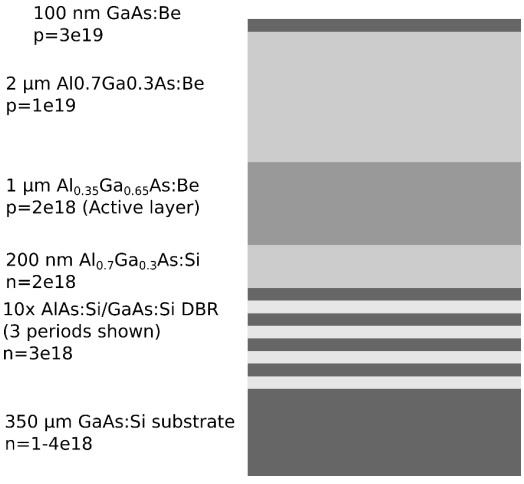
\includegraphics[width=0.45\textwidth]{figures/metal_layers.jpg}
    \caption{
        The layered LED sample made by the staff of the course.
        The layers were grown in the MBE, molecular beam epitaxy, machine at NTNU NanoLab.
        Figure borrowed from the lab manual \cite{labmanual}.
    }
    \label{fig:metal_layers}

\end{figure}

Each step was first done with a GaAs dummy sample to check that the process was working as intended.
After the last step, the LED was tested at a lab at IES, the Department of Electronic Systems at NTNU.


\subsection{LED design}
\label{methods:led_design}

Different finger spacings and finger widths were tested.
An overview schematic of the LED design is shown in \autoref{fig:led_schematic}.
One LED was 1 mm x 1 mm.
The bus bar for contact pad was 1 mm x 40 \textmu m.
The bus bar connecting the fingers was 1 mm x 30 \textmu m.
The fingers were 500 \textmu m long, with widths at 4, 8, 12 and 16 \textmu m, and finger spacings at 40, 60, 80 and 100 \textmu m.
The first lithography layer is shown in \autoref{fig:CleWin_L1}.
The second lithography layer, \autoref{fig:CleWin_L2}, was equal to the first, but scaled with a 5 \textmu m buffer everywhere to protect the fingers. 
The third lithography layer, \autoref{fig:CleWin_L3}, was for the mesa etch, and was a box around each LED with a 6 \textmu m buffer. 
The fourth lithography layer, \autoref{fig:CleWin_L4}, was for the etch of the passivation layer, and was a 30 \textmu m x 980 \textmu m box on each bottom bus bar. 
The fifth and final lithography layer, \autoref{fig:CleWin_L5}, was for the pad metallization, and was a 1000 \textmu m x 800 \textmu m box at the bottom of each LED connected to the bottom bus bar.
Schematics of the different layers are shown in \autoref{fig:CleWin_L1} to \autoref{fig:CleWin_L5}.
Schematics of the alignment marks in layer 1 and layer 2 is shown in \autoref{fig:CleWin_alignment_marks}.

\begin{figure}[ht]
    \centering
    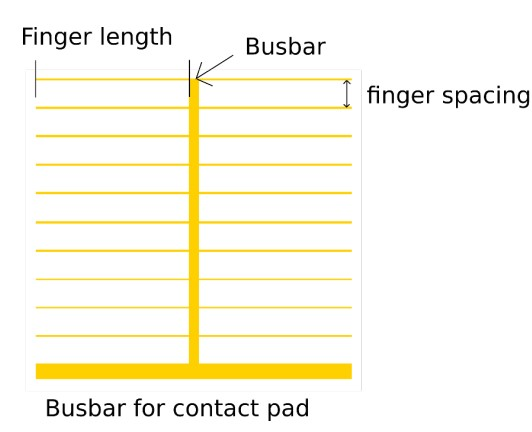
\includegraphics[width=0.45\textwidth]{figures/LED_schematic.jpg}
    \caption{
        Schematic of the LED design.
        Figure borrowed from the lab manual.
    }
    \label{fig:led_schematic}
\end{figure}

% clewin figures, L1 to L5 and alignment marks


\begin{figure}[ht]
    \centering
    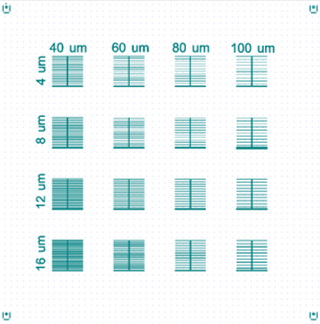
\includegraphics[width=0.45\textwidth]{figures/CleWin_L1.png}
    \caption{
        Layer 1. 
        Numbers on the top is the spacing between the fingers in the LED matrix.
        Numbers on the left side is the width of the fingers in the LED matrix.
        Each LED is 1 mm x 1 mm. 
        Alignment marks for layer 1 are in the corners. 
    }
    \label{fig:CleWin_L1}
\end{figure}


% L2
\begin{figure}[ht]
    \centering
    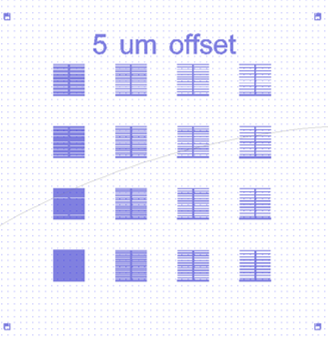
\includegraphics[width=0.45\textwidth]{figures/CleWin_L2.png}
    \caption{
        Layer 2. 
        This is the same as layer 1, but with a 5 \textmu m buffer on the whole pattern. 
    }
    \label{fig:CleWin_L2}
\end{figure}


% L3 
\begin{figure}[ht]
    \centering
    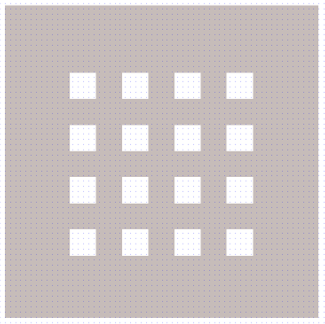
\includegraphics[width=0.45\textwidth]{figures/CleWin_L3.png}
    \caption{
        Layer 3. 
        This is the mesa etch layer. 
        The size of the box covering each LED is 1.012 mm x 1.012 mm.
    }
    \label{fig:CleWin_L3}
\end{figure}

% L4
\begin{figure}[ht]
    \centering
    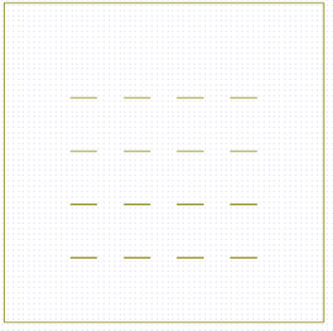
\includegraphics[width=0.45\textwidth]{figures/CleWin_L4.png}
    \caption{
        Layer 4. 
        This is the HF etch layer. 
        Each bar is covering a part of the bottom bus bar, with a size of 30 \textmu m x 980 \textmu m.
    }
    \label{fig:CleWin_L4}
\end{figure}

% L5
\begin{figure}[ht]
    \centering
    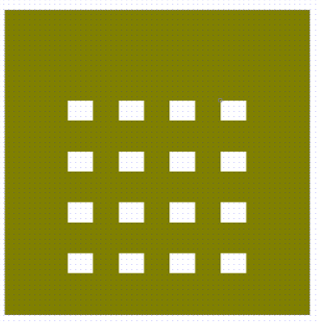
\includegraphics[width=0.45\textwidth]{figures/CleWin_L5.png}
    \caption{
        Layer 5. 
        This is the pad metallization layer, where each box is 1 mm x 0.8 mm. 
        The box is covering the bottom bus bar of each LED. 
    }
    \label{fig:CleWin_L5}
\end{figure}


% Alignment marks
\begin{figure}[ht]
    \centering
    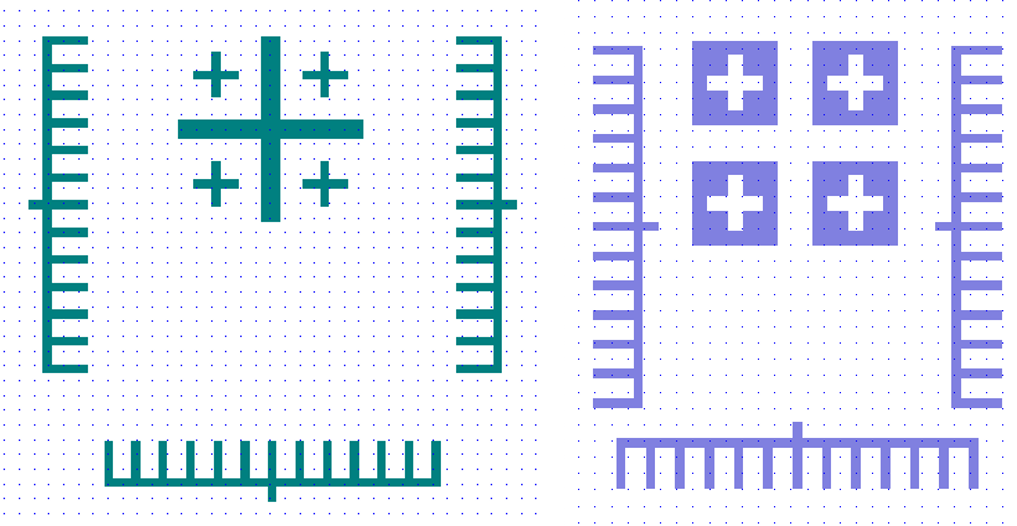
\includegraphics[width=0.45\textwidth]{figures/CleWin_alignment_marks.png}
    \caption{
        Alignment marks for layer 1 on the left and layer 2 on the right. 
        The design allows quantification of the alignment error.
        These marks are the Verniers design. 
    }
    \label{fig:CleWin_alignment_marks}
\end{figure}




\subsection{Front contact formation}
\label{methods:front_contact}

The bus bars and their fingers, i.e. the front contacts, were formed with lithography and lift-off.
A dose test was done to find the optimal dose and developing time for the resist, ensuring an undercut.
To verify this, both a SEM image and optical images of the sample were taken.
The optimal dose for MAN 440 was 1300 mJ/cm$^2$ and the optimal developing time was 5 minutes.
The hot plate temperatures are from the NanoLab hot plates in the student lab area, which have not been calibrated in a long time and can have some uncertainties. 
Negative photoresist was used, and the steps were done in the following order:
\begin{enumerate}
    \item Cleaned the sample with acetone and IPA.
    \item Dehydration baked at 150 \textdegree C for 5 minutes.
    \item Spin coated MAN 440 resist at 4000 rpm for 30 seconds with 1000 rpm/s acceleration.
    \item Cleaned the backside.
    \item Soft baked at 95 \textdegree C for 1 minute.
    \item Exposed the pattern at 1300 mJ/cm$^2$ in the MLA, maskless aligner.
    \item Developed in maD-332S developer for 5 minutes.
    \item Optical inspected the pattern.
    \item Teaching assistants metallized the wafer with a Pd/Ti/Pt/Au stack.
    \item Lift-off with acetone.
\end{enumerate}

The Pd/Ti/Pt/Au stack is referred to as the Au fingers. 

Unfortunately, a mix-up of the type of developer was done, and the process had to be repeated. 
The optical inspection before round number two showed some contamination on the wafer, which was probably caused by the wrong developer.
The wafer was cleaned thoroughly with acetone and IPA before the second round, but some contamination might have been left behind.

Another problem was that the dose test were done with a resist that got emptied, and a newer resist had to be used for the actual process.
When using the new resist the developer time was increased from 5 to 6 minutes, which gave an undercut but damaged the alignment marks and the thickest and closest fingers.




\subsection{GaAs contact layer etch}
\label{methods:wet_etch}
The heavily p-doped GaAs layer at the top of the metal stack was etched away to allow light to pass out of the LED.
The deposited Au fingers were measured to be 250 nm high in the profilometer.
Measuring the Au height was important for the later measurement of the etch depth of the 100 nm GaAs layer.
The Au fingers were protected with a positive photoresist before the wet etch.
Optimal dose for the positive photoresist was found to be 130 mJ/cm$^2$.
The preperation was done with the following steps:
\begin{enumerate}
    \item Cleaned the sample with IPA.
    \item Dehydration baked at 115 \textdegree C for 5 minutes.
    \item Spin coated SPR 700 resist at 4000 rpm for 34 seconds with 1000 rpm/s acceleration.
    \item Soft baked at 95 \textdegree C for 1 minute.
    \item Aligned the pattern in the MLA. The alignment marks were badly damaged, so the alignment was not perfect. % See \autoref{fig:align_marks}.
    \item Exposed the pattern at 130 mJ/cm$^2$ in the MLA.
    \item Post exposure baked at 115 \textdegree C for 1 minute.
    \item Developed in maD-332S developer for 30 seconds.
    \item Optical inspected the pattern to see if it covered the Au fingers.
\end{enumerate}

Quantification of the misalignment with the Verniers were tried, but the Verniers were too badly damaged to get any number out.
The wet etch was done at the chemical clanroom at NTNU NanoLab, with NH$_3$:H$_2$O$_2$:H$_2$0 in 3:1:300 ratio.
The ammonium hydroxide was 30\%.
The etch depth was tested on the GaAs dummy sample, and measured with the profilometer to figure out an etch time which would remove 100 nm of GaAs.
The GaAs dummy was etched 50 nm at the first run, thus the time was doubled for the LED etch to achieve 100 nm.
The etch steps were as follows:

\begin{enumerate}
    \item 3 mL 30\% NH$_3$ was added to the etch tank with 300 ml H$_2$O.
    \item 1 mL H$_2$O$_2$ was added to the etch tank.
    \item The sample was placed in the etch tank for 90 seconds.
    \item The sample was rinsed with H$_2$O and cleaned on the backside.
    \item The protective photoresist was removed with acetone and IPA before profilometer measurement.
    \item The etch depth was measured with the profilometer.
\end{enumerate}



\subsection{Backside contact formation}
\label{methods:backside_metallization}
The backside of the LED sample was metallized with a Pd/Ge/Ti/Pt/Au stack to form the backside contact.
The positive photoresist SPR 700 was used to protect the frontside, using the following steps:
\begin{enumerate}
    \item Cleaned the sample with acetone and IPA.
    \item Dehydration baked at 115 \textdegree C for 5 minutes.
    \item Spin coated SPR 700 resist at 4000 rpm for 34 seconds with 1000 rpm/s acceleration.
    \item Soft baked at 95 \textdegree C for 1 minute.
    \item No exposure was done, since the whole frontside needed to be protected.
    \item Post exposure baked at 115 \textdegree C for 1 minute.
    \item Developed in maD-332S developer for 30 seconds.
    \item Optically inspected the pattern to see if the whole frontside was covered.
    \item Backside metallization was done by the teaching assistants.
\end{enumerate}


\subsection{Mesa etch, PECVD passivation deposition, and contact annealing}
\label{methods:PECVD}
In one session the the mesa was etched, the passivation layer deposited and the contacts annealed.
The mesa etch was done with a wet etch with H$_3$PO$_4$:H$_2$O$_2$:H$2$O 5:5:15, with the goal of separating the 16 LEDs.
The mesa etch had to get through the two p-doped Al$_{0.7}$Ga$_{0.3}$As layers, i.e. had to be deeper than 3 \textmu m.
The preperation for the mesa etch was to add a positive photoresist mesa mask, which was done in the following steps:

\begin{enumerate}
    \item Cleaned the sample with acetone and IPA.
    \item Dehydration baked at 115 \textdegree C for 5 minutes.
    \item Spin coated SPR 700 resist at 4000 rpm for 34 seconds with 1000 rpm/s acceleration.
    \item Soft baked at 95 \textdegree C for 1 minute.
    \item Aligned the pattern in the MLA.
    \item Exposed the pattern at 130 mJ/cm$^2$ in the MLA.
    \item Post exposure baked at 115 \textdegree C for 1 minute.
    \item Developed in maD-332S developer for 30 seconds.
    \item Optically inspected the pattern to see if it covered the LEDs.
\end{enumerate}

The mesa etch and passivation deposition was done in parallel.
The wet etch was first done on the GaAs dummy to test the etch time, where it was found that 1 minute 30 seconds would be sufficient to etch through the two p-doped layers.
The thickness aim for the passivation layer was 253 nm. 
The following steps were done:

\begin{enumerate}
    \item Deposited Si$_3$N$_4$ passivation layer on Si to find an optimal layer thickness. The recipe used was "(OPT) Si3N4" for 18 minutes and 35 seconds.
    \item Wet etched the dummy to find a suitable etch time. This etch time was 1 minute 15 seconds, which was increased by 15 seconds for the LED etch.
    \item The wet etch was done with H$_3$PO$_4$:H$_2$O$_2$:H$2$O 5:5:15 mL.
    \item The resist was stripped of the dummy, and the etch depth was measured with the profilometer.
    \item The inferometer was used to measure the passivation layer deposition thickness.
    \item The LED was mesa wet etched as the dummy was, but with 1 minutes 30 seconds etch time.
    \item The etch depth was controlled to be deeper than 3 \textmu m in the profilometer.
    \item PECVD passivation layer deposition was done on the LED and the dummy with the same recipe and time as the Si test, because the recipe was found to be good enough.
    \item The last step was the contact annealing, which was done with warm up to 420 \textdegree C, and 30 seconds annealing at 420 \textdegree C, before cooling down to room temperature.
\end{enumerate}



\subsection{Planarization and passivation layer etch}
\label{methods:Planarization}

The passivation layer HF etch was done by the teaching assistants.
The planarization and preperation for the passivation layer etch was to add a thick positive photoresist with a mask opening on the bottom bus bar, and was done in the following steps:

\begin{enumerate}
    \item Cleaned the sample with acetone and IPA.
    \item Dehydration baked at 150 \textdegree C for 5 minutes.
    \item Spin coated AZ5214E positive resist at 1000 rpm for 34 seconds with 250 rpm/s acceleration.
    \item Soft baked at 95 \textdegree C for 1 minute.
    \item Exposed the pattern at 80 mJ/cm$^2$ in the MLA.
    \item Developed in 70:30 ma-D 332S:H$_2$O developer for 1 minute 30 seconds.
    \item Hard baked at 175 \textdegree C for 15 minutes.
    \item Optical inspection of the pattern.
    \item Teaching assistants preformed HF etch to expose the Au in the bottom bus bar.
\end{enumerate}



\subsection{Pad metallization}
\label{methods:pad_metallization}

Lithography on the LED sample was done to prepare for the pad metallization.
The teaching assistants did the pad metallization.
The preparation was to make a negative photoresist mask for the pad metallization, and was done in the following steps:
\begin{enumerate}
    \item Cleaned the sample with IPA.
    \item Dehydration baked at 115 \textdegree C for 5 minutes.
    \item Spin coated MAN 440 resist at 4000 rpm for 30 seconds with 1000 rpm/s acceleration.
    \item Soft baked at 95 \textdegree C for 1 minute.
    \item Exposed the pattern at 1300 mJ/cm$^2$ in the MLA
    \item Developed in maD-332S developer for 5 minutes.
    \item Optical inspected the pattern to see if the pattern covered the bottom bus bar and an area below.
    \item Handed in the sample to the teaching assistants, who did the pad metallization with Ti/Au, with 30 nm Ti and 500 nm Au.
    \item Lift-off was done with acetone.
\end{enumerate}


\subsection{LED testing/characterization}
\label{methods:LED_testing}

The final LED sample was tested using a Keithley 2450 SourceMeter, a probe, and an optical microscope.
Initially, there was no measured contact in the LED between the frontside and the backside.
The voltage was then turned up to 10 V, which warmed up the LED and gave contact. 
Using the SourceMeter, the voltage was swept from -1 V to 3 V, while the measured current was recorded.
The measuring was automatically stopped when a current of 30 mA was reached.
The results were then plotted as an IV-curve.
Two of the LEDs was measured this way. 

The LED was turned on with 1.71 V and 30 mA, and images was taken with an iPhone.

%%%%%%%%%%%%%%%%%%% RESULTS %%%%%%%%%%%%%%%%%%
\section{Results}
\label{results}
% RESULTS


put in figures and shit.

We still need the following:
% list
\begin{itemize}
    \item images of allingment marks
    \item ?
\end{itemize}


%%%%%%%%%%%%%%%%%%% DISCUSSION %%%%%%%%%%%%%%%%%%
\section{Discussion}
\label{discussion}
% DISCUSSION

\subsection{Photolithography}
\label{sec:discussion:photolithography}

% lithography undercut 
All the lithography processes used in this work gave valuable experience.
One of the experiences was how to do a dose test to get a sufficient undercut while using negative photoresist. 
The lab manual for the course \cite{labmanual} states that the undercut should be at least 1 \textmu m deep, while the teaching assistant stated that 0.5-1 \textmu m would be sufficient.
Getting an exact measurement of the undercut was difficult with the Table Top SEM, because the tilting and rotation of the sample in the chamber is very restricted. 
Quantification of the undercut is problematic with the Table Top SEM, but the undercut is clearly visible in the SEM image in \autoref{fig:undercut}.
Estimating the undercut was easier when using the optical microscope. 
First it was assessed whether the slope visible in the optical images in \autoref{fig:undercut_top} and \autoref{fig:undercut_bot} was an undercut or not.
Over- and under focusing on the edge indicated that the slope was an undercut, and this was confirmed in the SEM. 
The quantification of the undercut was done by measuring the length of the slope and comparing this to the width of the finger. 
This is a crude approximation, but it confirmed that the undercut was in the range of 0.5-1.5 \textmu m, assuming that the widest part of the finger was 4 \textmu m wide.


% negative vs positive resist
If all the photolithography steps were done again, using only positive photoresist could have yielded better results.
The first layer made with negative photoresist produced many defect fingers, while the second layer made with positive photoresist on top of the fingers did not have the same defects.
Lift-off with positive photoresist is known to be possible with sufficiently large structures. 
Negative photoresist is normally used for lift-off, but results from this work suggests that trials with positive photoresist should be done for lift-off. 


\subsection{Etch}
\label{sec:discussion:etch}

% the etch curves which are not flat
The plots from the profilometer on the etches show that the etch is not perfectly flat.
Three artifacts have been identified in the etch process.

One artifact is the contact loss shown in \autoref{fig:Dummy_GaAs_80nm_etch_lost_contact}. 
Here the depth is measured to 330 nm, but this is uncertain since the contact is lost 20 \textmu m after the etch edge.
The contact loss can be countered with the right settings on the profilometer. 
The artifact could have been something else, but the contact loss is the most likely cause since the profilometer data outside the plot on the left side is flat and correct. 

A second artifact are on the vertical edges, where the etch is varying a lot. 
This is illustrated in \autoref{fig:profilometer_GaAs_100nm_etch}.
The other vertical edges varied in other but similar ways. 
This could both be caused by the etch process and the profilometer.
The profilometer might struggle to measure around vertical edges. 
The etch process could be affected by  the increased area and by different etch rates on different crystallographic planes.

A third artifact is the squiggly surface, shown between the fingers in \autoref{fig:profilometer_GaAs_100nm_etch}. 
This artifact is caused by the etch process, and is present all over the wafer where the etch was done. 
The surface is varying around $\pm$ 5 nm, which is a lot for a 100 nm etch.
This artifact could potentially block some of the light from the LED, but it is not clear how much of the light this could block.

\subsection{Deposition of passivation layer} 
If all process steps are done correctly, the LED will emit light at 675 nm.  
For Si$_3$N$_4$, this corresponds to an optical thickness of around 253 nm.
The optical thickness of Si$_3$N$_4$ was measured to be 249.70 nm and calculated to be 247.91 nm.
A few nanometers difference between the measured and calculated thickness is expected, because the $n$ in the calculation is an approximation. 
The values are very close to the target, which is good.

In order to adjust the thickness to get even closer to the target thickness, the deposition time could be adjusted.
The deposition time was 18 minutes and 35 seconds.
This corresponds to a deposition rate of 0.22 nm/sec, assuming that the deposition was linear and that the measured thickness is correct.
Using these numbers, the deposition time could be adjusted to 18 minutes and 50 seconds, which would give an optical thickness of 253.06 nm, slightly closer to target value.

%Adding a passivation layer % https://www.sciencedirect.com/topics/engineering/passivation-layer




\subsection{Surface artifact}
\label{sec:discussion:surface_artifact}

The surface of the LED sample was far from perfect throughout the process.
While alignment in the MLA was done, multiple surface impurities were visible. 
These impurities are probably what is seen as a high and abrupt peak in the profilometer data in \autoref{fig:profilometer_GaAs_100nm_etch} around 320 \textmu m.
Peaks like this one are visible in all the profilometer data from the sample. 
The optical microscope images in \autoref{fig:led_optical} show that the surface have many surface impurities which have cracked before, during or after annealing. 


The annealing process made the surface artifacts and more visible.
It is most likely that the surface impurities were present before the etch, and that the etch process has made the area around the impurities more susceptible to cracking and slightly different etch rates.
The different etch rates are visible as different colors in the optical microscope images in \autoref{fig:led_optical}, which can arise due to different thicknesses. 
Another argument for the artifacts being a result of the etch process and not the annealing, is that the passivation layer totally covers the surface and protects it from damage. 






%%%%%%%%%%%%%%%%%%% CONCLUSION %%%%%%%%%%%%%%%%%%
\section{Conclusion}
\label{conclusion}
% Conclusion

% This is the abstract

% Light emitting diodes (LED) are widely used light producing electrical components.
% % The production of such devices .... smt nanotechnology?
% In this rapport, a premade multi-layered semiconductor wafer is used to produce LEDs.
% The wafer have been processed by strategically using photolithography, deposition, and etching.
% The LED have been characterized using an optical microscope, a scanning electron microscope, a profilometer, an ellipsometer and a SourceMeter.
% Measurements of the IV-characteristics of the LEDs have been performed, which confirmed that the LEDs are working as a diode, and they are emitting light.
% With voltage at 1.7 V and current at 30 mA the LEDs emits red light, which is the around the target wavelength of 675 nm.


% This is the conclusion
Functioning LEDs have been produced by using a multi-layered semiconductor wafer.
The wafer have been processed by strategically using photolithography, deposition, and etching.
Characterization of the LEDs have been performed and the results show that the LEDs are working as a diode.
With voltage at 1.7 V and current at 30 mA the LEDs emits red light, which is the around the target wavelength of 675 nm.

%%%%%%%%%%%%%% REFERENCES %%%%%%%%%%%%%%%%%%
}
\begingroup
\begin{center}
  \rule{2cm}{.4pt}
\end{center}
\makeatletter
\@beginparpenalty=10000
\makeatother
\bibliographystyle{unsrt} %unsrtnat
\bibliography{references}


\endgroup

\end{document}